\documentclass[aspectratio=169,11pt]{beamer}
\usepackage[T1]{fontenc}
\usepackage{lmodern}
\usepackage{graphicx}
\usepackage{booktabs}
\newcommand{\TitleMain}{Walk calibration of BTL modules in testbeam:}
\newcommand{\TitleSub}{Via Synchronization of MCP scope data with FEBd}
\newcommand{\ShortTitle}{MCP synchronization and walk calibration}

% Generated from frozen numerical results by build_assets.py.
\newcommand{\TimingCount}{10127}
\newcommand{\DBefore}{55.16}
\newcommand{\DAfter}{54.82}
\newcommand{\DLow}{54.32}
\newcommand{\DHigh}{55.22}
\newcommand{\DSD}{61.26}
\newcommand{\DTail}{1.57}
\newcommand{\RBefore}{77.69}
\newcommand{\RAfter}{64.16}
\newcommand{\RLow}{63.27}
\newcommand{\RHigh}{64.99}
\newcommand{\RSD}{70.33}
\newcommand{\RTail}{1.56}
\newcommand{\RefBinsA}{19}
\newcommand{\RefBinsB}{19}
\newcommand{\RefBinsC}{20}
\newcommand{\RefBinsD}{19}
\newcommand{\ExampleAWC}{18.332}
\newcommand{\ExampleLow}{18.120}
\newcommand{\ExampleHigh}{18.607}
\newcommand{\ExampleRMS}{6.80}
\newcommand{\GapCount}{703}
\newcommand{\SummaryChi}{538.6}
\newcommand{\PredictorRMSE}{3.22}
\newcommand{\PredictorFraction}{14.1}

\usetheme{default}
\setbeamercolor{normal text}{fg=black,bg=white}
\setbeamercolor{structure}{fg=black}
\setbeamersize{text margin left=7mm,text margin right=7mm}
\setbeamertemplate{navigation symbols}{}
\setbeamerfont{frametitle}{size=\large,series=\bfseries}
\setbeamertemplate{headline}{%
  \hbox to \paperwidth{\hspace{7mm}\scriptsize\color{black!55}Internal review draft -- 22 October 2026
  \hfill\raisebox{0pt}[9mm][1mm]{
\includegraphics[height=7mm]{CMSlogo_black_label_1024.png}}\hspace{6mm}}}
\setbeamertemplate{footline}{%
  \hbox to \paperwidth{\hspace{7mm}\scriptsize\ShortTitle
  \hfill V2 slides -- draft 1\quad\insertframenumber/\inserttotalframenumber\hspace{7mm}}\vspace{2mm}}
\setbeamertemplate{frametitle}{\vspace{-1mm}\insertframetitle\par\vspace{1mm}}
\setlength{\parskip}{4pt}
\newcommand{\Code}[2]{\href{https://github.com/De-Cristo/LecroyTranslator4CMSTimingDetector/blob/45a907c422d6c8afbe0cdf44cd2827d3433d0f97/#1}{#2}}
\newcommand{\Source}[1]{\par\smallskip{\fontsize{8}{9.5}\selectfont\color{black!65}#1\par}}
\newcommand{\PlotSlide}[4]{%
  \begin{frame}[t]{#1}
  \begin{columns}[T,onlytextwidth]
    \begin{column}{.63\textwidth}
      \centering\includegraphics[width=\linewidth,height=51mm,keepaspectratio]{figures/#2.pdf}
    \end{column}
    \begin{column}{.35\textwidth}\fontsize{10}{12}\selectfont #3\end{column}
  \end{columns}
  \Source{#4}
  \end{frame}}
\newcommand{\TitleSlide}{%
  \begin{frame}
    \centering{\Large\TitleMain\par}\vspace{3mm}
    {\large\TitleSub\par}\vspace{8mm}
    {\large CMS\par}\vspace{2mm}
    \href{mailto:cms-dpg-conveners-mtd@cern.ch}{cms-dpg-conveners-mtd@cern.ch}
    \vspace{7mm}\par{\small Discussion draft; not approved for public release.}
  \end{frame}}
\hypersetup{pdftitle={\TitleMain\space\TitleSub},pdfauthor={CMS}}

\begin{document}
\TitleSlide

\begin{frame}{Purpose: provide a reliable time reference for BTL analyses}
\large
Several BTL test-beam analyses need a reliable particle-arrival time reference.
\medskip

For a subset of the data, a digital oscilloscope recorded MCP-PMT signals
in parallel with the BTL readout.
\medskip

\textbf{Approach:} synchronize the two streams, use the MCP to calibrate
upstream reference bars, then use their corrected times as the reference
for downstream timing.
\medskip

\normalsize
\textbf{Final check:} the time difference between downstream and reference bars
before and after walk correction.
\end{frame}

\PlotSlide{Parallel MCP and BTL streams are linked through FEBd}{setup}{
\textbf{Two readout streams}

The scope records the MCP-PMT pulse. FEBd records the BTL SiPM signals.

\textbf{Synchronization link}

The scope trigger also reaches TOFHIR channel 192 in FEBd.

This link connects independently clocked records of the same particle.
}{September 2025 beam test. The highlighted lower path provides the reference-bar data.
This FEBd-based synchronization is specific to the test-beam setup, not the final HL-LHC synchronization scheme.}

\PlotSlide{Events are correlated using the intervals between triggers}{event_matching}{
\begin{enumerate}
\item Compare consecutive trigger intervals in channel 192 and the scope.
\item Find consistent interval patterns.
\item Keep only unique event matches.
\end{enumerate}

Consistent trigger patterns identify coincident events in the two streams.

Event matching alone does not remove relative clock drift.
}{The correlated intervals and their ratio test event matching, not detector resolution.
\Code{FEBD_Sync/simple_sync.py}{GitHub: trigger matching}.}

\PlotSlide{The matched clocks show low-frequency relative drift}{clock_residuals}{
\textbf{Correct the timing coordinate}

\begin{enumerate}
\item Split data at clock resets.
\item Fit a line between matched trigger times in each segment.
\item Fit the remaining drift with LOWESS.
\end{enumerate}

Add the drift to the line prediction to obtain $g(u)$, the expected TOFHIR trigger time.
}{Points show residuals before LOWESS; red curves describe smooth drift.
Reject groups with pre-LOWESS residual scale $1.4826\,\mathrm{MAD}>1$\,ns.
\Code{TimeCalibration/ch192_vs_trigger_lowess.py}{GitHub: clock reconstruction}.}

\PlotSlide{After synchronization, the MCP defines the calibration time}{mcp_waveform}{
Fit the MCP waveform to estimate its pulse time.

Within the scope waveform, define
\[
\delta_{\rm MCP}=t_{\rm peak}-t_{\rm trigger}.
\]
For SiPM channel $i$, use
\[
\Delta t_i=t_i-g(u)-\delta_{\rm MCP}.
\]
The charge-dependent part of this difference is the walk.
}{The waveform and fitted template determine the MCP pulse time. $u$ is the scope-trigger timestamp.
A fixed cable/geometry offset is irrelevant to the shape; clock-rate conversion over the short waveform interval is neglected.}

\begin{frame}{Measure the upstream channels' time walk versus charge}
\small
Measure the charge-dependent threshold delay relative to the synchronized MCP.
\begin{enumerate}
\item In run 4399, require exactly five TOFHIR hits and a unique MCP match:
the target upstream pair, downstream channels 234 and 243, and channel 192.
\item Require waveform and clock quality, finite positive charge and slope-quality quantities.
Keep charge at or above the spectrum's left half-maximum boundary.
\item Form 20 uniform $1/Q$ bins. Clip timing outliers at
$5(1.4826\,\mathrm{MAD})$ from each bin's median; require at least five entries.
\item Fit the bin means with weights $1/\mathrm{SEM}^2$:
\[
W_i(Q)=a_i+b_i/Q+c_i/Q^2.
\]
\end{enumerate}
$Q$ is the measured ADC charge proxy, not energy in MeV.
SEM denotes the standard error of the mean.
\Source{Reference pairs: bar 7 = channels 133 and 154; bar 8 = channels 137 and 150.
\Code{Q_Walk/qwalk_t0_data.py}{GitHub: selected reference sample}.}
\end{frame}

\begin{frame}[t]{Walk-corrected upstream bars provide the time reference}
\begin{columns}[T,onlytextwidth]
\begin{column}{.49\textwidth}
\centering\textbf{Bar 7: channel 154}\par
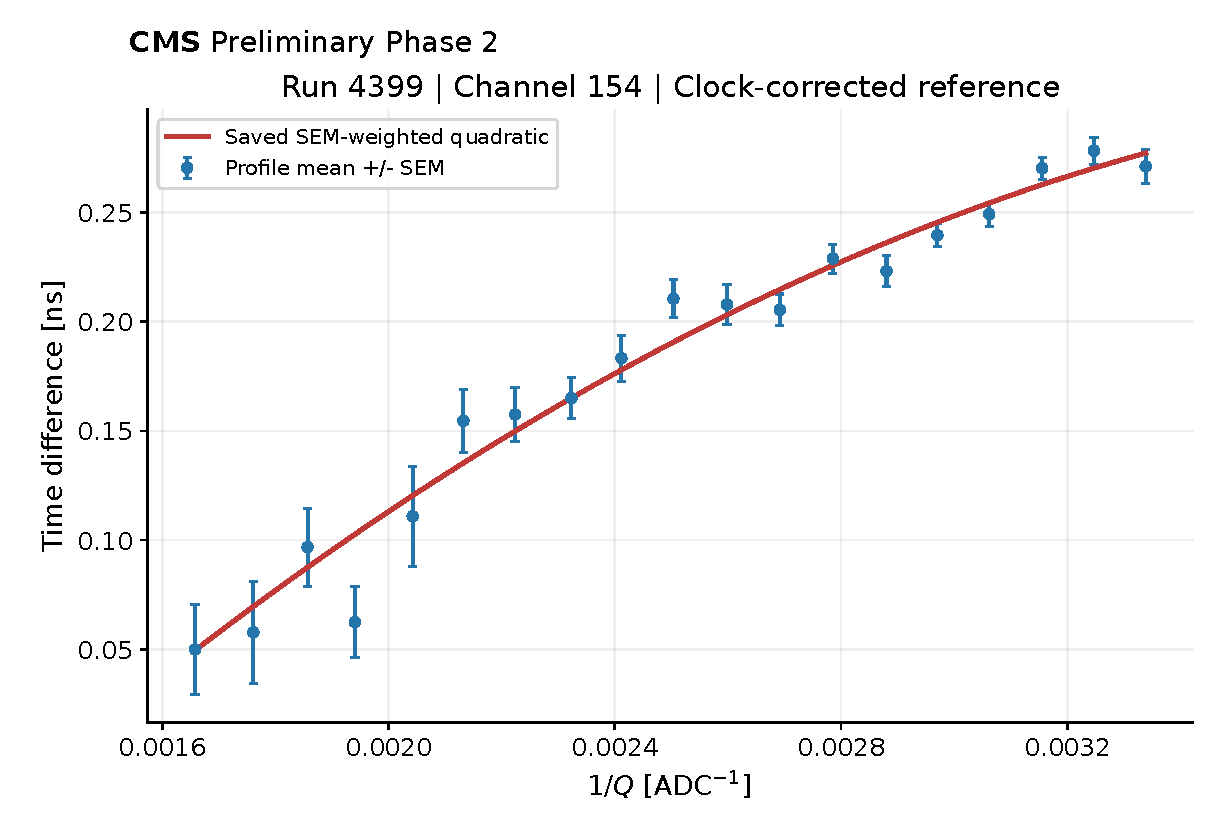
\includegraphics[width=\linewidth,height=43mm,keepaspectratio]{figures/clock_reference_ch154.pdf}
\end{column}
\begin{column}{.49\textwidth}
\centering\textbf{Bar 8: channel 137}\par
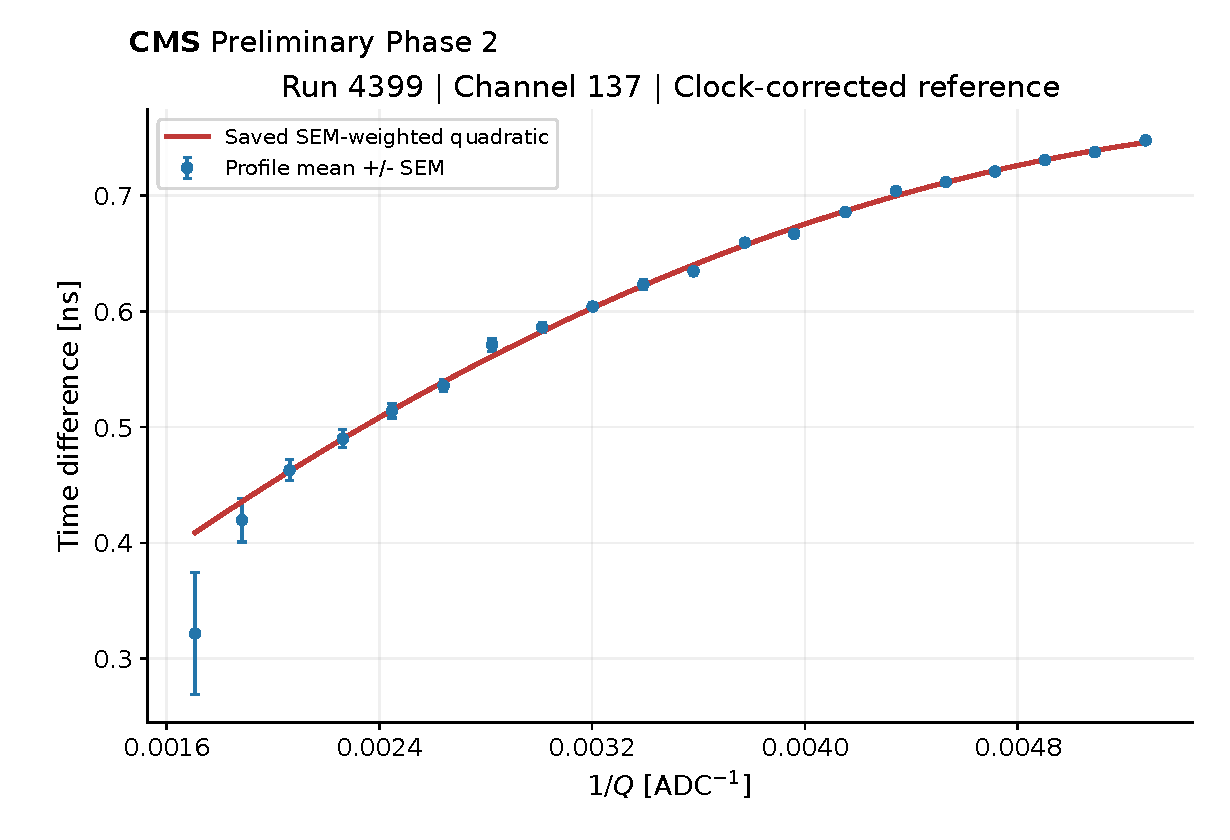
\includegraphics[width=\linewidth,height=43mm,keepaspectratio]{figures/clock_reference_ch137.pdf}
\end{column}
\end{columns}
\small
Correct each end: $t_i^{\rm corr}=t_i-W_i(Q_i)$.
Use the bar average: $t_{\rm ref}=(t_L^{\rm corr}+t_R^{\rm corr})/2$.
\Source{Run 4399 examples. Points show mean time differences with SEM; red curves are SEM-weighted quadratics in $1/Q$.
Only populated charge support is shown. The +26\,ns display offset does not change the walk shape.
The full note also shows channels 133 and 150.}
\end{frame}

\PlotSlide{Check the calibrated reference bar against the MCP}{validated_bar_mcp}{
\textbf{\TimingCount{} common events}

Subtract each channel's fitted walk, then form the bar-average time minus MCP time.

\textbf{Core width}
\[
\RBefore\ \longrightarrow\ \RAfter\ \mathrm{ps}
\]
Corrected full-sample SD: \RSD\,ps.

This is not the intrinsic bar resolution.
}{Fixed clock mapping; a truncated-normal core fit uses median $\pm2.5(1.4826\,\mathrm{MAD})$.
The corrected-width 16--84\% interval is [\RLow, \RHigh]\,ps from 400 file/segment-block bootstraps with fixed calibrations.}

\PlotSlide{Final check: downstream--reference-bar timing}{bar_pair_before_after}{
\textbf{8,737 common events}

Bar 3 (234, 243) minus reference bar 8 (137, 150).

All four channels are walk corrected before averaging each bar's ends.

\textbf{Core width}
\[
161.7\ \longrightarrow\ 141.8\ \mathrm{ps}
\]
\textbf{12.3\% narrower.}
The MCP time cancels from this difference.
}{Same events and populated charge support; histograms median-centered for display.
Same core-fit definition as the preceding slide; fixed-calibration 68\% block interval: [138.0, 145.6]\,ps after correction.
In-sample, asymmetric and fit-window dependent; not a single-bar resolution measurement.}
% Original entries except Saclay; MCP journal citation updated by author request.
\begin{frame}[t]{References}
\fontsize{7.5}{8.8}\selectfont
\setlength{\parskip}{0pt}
\setbeamertemplate{bibliography item}[text]
\begin{columns}[T,onlytextwidth]
\begin{column}{.485\textwidth}
\begin{thebibliography}{7}
\setlength{\itemsep}{3pt}
\bibitem[1]{github_repo}
GitHub repository,
\url{https://github.com/De-Cristo/LecroyTranslator4CMSTimingDetector}.
\bibitem[2]{picosec}
J. Bortfeldt et al., ``Timing Performance of a Micro-Channel-Plate Photomultiplier Tube'',
\href{https://doi.org/10.1016/j.nima.2020.163592}{Nucl. Instrum. Meth. A \textbf{960} (2020) 163592}
[\href{https://arxiv.org/abs/1909.12604}{arXiv:1909.12604}].
\bibitem[3]{MTDTDR}
CMS Collaboration, ``A MIP Timing Detector for the CMS Phase-2 Upgrade''.
Technical Report CERN-LHCC-2019-003. CMS-TDR-020, CERN, Geneva, 2019 and
``A High-Granularity Timing Detector for the ATLAS Phase-II Upgrade'',
CERN-LHCC-2020-007; ATLAS-TDR-031
\end{thebibliography}
\end{column}
\begin{column}{.485\textwidth}
\begin{thebibliography}{7}
\setlength{\itemsep}{3pt}
\bibitem[4]{WhitePresentation}
S. White, Nov. 2025 BTL TB Analysis mtg presentation,
\url{https://indico.cern.ch/event/1614521/contributions/6803723/attachments/3178820/5922530/5vs10vs20GSa_s.pdf}
\bibitem[5]{Leo}
W. R. Leo, ``Techniques For Nuclear and Particle Physics Experiments'',
p.326, Springer-Verlag Berlin Heidelberg.
\bibitem[6]{DualThreshold}
S. White and A. Boletti, ``Amplitude Walk in Fast Timing: The Role of Dual Thresholds''
2026 JINST V21 P02001.
\bibitem[7]{LOWESS}
W. S. Cleveland, ``Robust Locally Weighted Regression and Regression Scatterplots'',
J. Amer. Statist. Assoc. \textbf{74} (1979) 829.
\end{thebibliography}
\end{column}
\end{columns}
\end{frame}

\end{document}
